\chapter{Reducing the number of explanatory variables}
\label{ch:ReducingTheNumberOfExplanatoryVariables}

\section{Introduction}
The explanatory variables used in SDMs are often correlated. Highly correlated variables can be an indication of redundant information in the data-set. Moreover, irrelevant predictors might be included into the model since there is usually no knowledge about which variables make up the niche. It is well known that this can lead to over-fitting and unstable predictions. In this chapter we describe some methods to deal with large sets of correlated predictors. More specifically, in Section \ref{sec:DimensionalityReduction} we introduce methods that transform the input space. In Section \ref{sec:Regularization} techniques that penalize ``large'' models are introduced. Finally, Section \ref{sec:SubsetSelectionMethods} deals with step-wise variable selection methods. \\

For a review of methods to deal with correlated covariates in ecology we refer to \cite{dormann_collinearity:_2013}. Finally, these automatic selection procedures are of course not meant to replace a well founded motivation of why certain predictors should be selected. A discussion of how the available data, scale of the predictors, etc.\ should influence the decision of using a complex or a simple model can be found in \cite{merow_what_2014}.

\section{Dimensionality reduction}
\label{sec:DimensionalityReduction}
Dimensionality reduction techniques can be used to obtain a new, often lower-dimensional, representation of important structures in the input space. This can be particularly useful when two or more explanatory variables are proxies of one underlying latent variable. For example, there are multiple indices that indirectly measure the amount of vegetation. A combination of these indices might be a better indicator of the amount of vegetation than the individual indices. The dimensionality reduction techniques that are used in this thesis use only the input space and ignore the outcome values. It should however be noted that there are other dimensionality reduction techniques that do take into account the relationship between input and output variables, e.g.\ partial least squares \parencite[see e.g.][]{marx_iteratively_1996}.

\subsection{Principal component analysis}
Often principal component analysis (PCA) is introduced as a method which constructs uncorrelated linear combinations of the variables, these new variables are called principal components. However, for our purposes it might be more interesting to view PCA as a way to find a low dimensional affine subspace such that when the original data is projected onto this subspace the ``information loss'' is minimal. One possible characterization of PCA is that a set of $K$ orthonormal vectors $\bm{u}_i$ and an offset vector $\bm{b}$ are constructed so that
\[\sum_{i=1}^{N} \sum_{j=1}^{K} \vert \vert \bm{x}_i - \bm{x}_i^t \bm{u}_i\bm{u}_i - \bm{b} \vert \vert_2^2 \]
is minimized. It can be shown that for a certain $K$ this sum is minimized when the $\bm{u}_i$ are the eigenvectors corresponding with the $K$ largest eigenvalues of the covariance matrix. A prototype scenario is shown in Figure \ref{fig:PCA}.\\

\begin{figure}[!htb]
\centering
\includegraphics[scale=0.5]{VectorGraphics/PCA.png}
\caption{\label{fig:PCA}Visualization of the a typical scenario where PCA is useful.}
\end{figure} 


Once the principal components have been obtained they can be used as the explanatory variables in one of the models of Chapter \ref{ch:ClassificationTechniques}. Since the new variables are uncorrelated and some irrelevant noise in the predictors might be removed the resultant models often exhibit less variance. \\

There are multiple criteria based upon which the number of principal components, $K$, can be chosen. One possibility is to plot the so-called ``explained'' variance versus the number of components and look for either a kink or a point where a certain percentage of variance is explained. If PCA is combined with a classification method it is usually more appropriate to use cross-validation to select the number of principal components. We will use the cross-validation approach.\\

It should be clear that the main disadvantage of PCA is that it only allows for linear representations of the data. Hence, PCA will often be useless if the observations are scattered around a non-linear manifold. For example in Figure \ref{fig:PCACircle} there is a clear underlying space that is one dimensional. However, using the first principal component of this fictional data-set would lead to as big an ``information'' loss as using just one of the original axes. For the sake of completeness we mention that there are extensions of PCA that use non-linear manifolds instead of linear ones, e.g.\ principal curves and surfaces \parencite{hastie_principal_1989}. \\

\begin{figure}[!htb]
\centering

\includegraphics[scale=0.5]{VectorGraphics/PCACircle.png}
\caption{\label{fig:PCACircle}Visualization of the a scenario where PCA is useless.}
\end{figure}



\subsection{Kernel principal component analysis}
A popular and computationally efficient non-linear dimensionality reduction technique is kernel PCA \parencite{scholkopf_kernel_1997}. In kernel PCA the elements of the input space $\mathcal{X}$, in our case we have $\mathcal{X} = \mathbb{R}^p$, are mapped to a Hilbert space $F$. We will denote the map as: 
\[\bm{\phi}(\cdot): \mathcal{X} \to F.\]
In this new vector space a PCA is conducted and new coordinates are obtained. A visual presentation of these steps is given in Figure \ref{fig:KernelPCA}. \\
\begin{figure}[!htb]
\centering
\includegraphics[scale=0.5]{VectorGraphics/KernelPCA.png}
\caption{\label{fig:KernelPCA}Visualization of kernel PCA.}
\end{figure}

One attractive property of kernel PCA is that we do not need to actually compute $\phi(\bm{x})$. More specifically we only need to compute the so-called kernel matrix $\mathbb{K}$
\[\mathbb{K}_{ij} = \langle \bm{\phi} (\bm{x}_i), \bm{\phi} (\bm{x}_j)  \rangle = k(\bm{x}_i,\bm{x}_j).\]
In general it can be shown that, under some regularity conditions, for any kernel function
\[k(\cdot,\cdot): \mathcal{X} \times \mathcal{X} \to \mathcal{R}\] 
there exists a corresponding $\bm{\phi}(\cdot)$ and Hilbert space $F$. Hence usually one specifies the kernel function instead of the map $\bm{\phi}(\cdot)$.\\ 

Popular kernel functions are:
\begin{itemize}
\item The polynomial kernel $k(\bm{x},\bm{y}) = (\bm{x}^t \bm{y} + c)^d$.
\item The radial basis kernel (RBF kernel) $k(\bm{x},\bm{y}) = \exp{\left(-\frac{\vert \vert \bm{x} -\bm{y}\vert \vert ^2}{\sigma}\right)}$, with $\sigma > 0$. 
\item The hyperbolic tangent kernel, $k(\bm{x},\bm{y}) = \tanh{(\sigma \bm{x}^t \bm{y} + c)}$.
\end{itemize}
In these representations the $\sigma$, resp.\ $c$, parameter can be seen as a scale, resp.\ offset, parameter. The value of these parameters is in general selected by using cross validation. We will focus on the RBF kernel, this kernel is usually used when no prior information is available \parencite{JSSv011i09}.  \\

A disadvantage of kernel PCA is that it is not always clear which kernel should be used. For our goals, combining kernel PCA and a classification method, we can use cross-validation and treat the type of kernel as a tuning parameter. Furthermore, it is not always particularly clear what the new features are supposed to represent (we might not even know in which Hilbert space we are working). An R implementation of kernel pca is provided as part of the \textsc{kernlab} package \parencite{JSSv011i09}.

\subsection{Presence versus background data}
\label{sec:dimRedPrVSBG}
In this section we focus on PCA but all the comments readily apply to kernel PCA.\\

When PCA is combined with classification techniques one usually performs the PCA on the predictor values of all the included cases. However, in presence-only models the background points are randomly generated and the number of these points can be chosen. It should be clear that when the number of background points approaches infinity the covariance matrix used in the PCA converges to the covariance matrix of the explanatory data within the study extent. Unless the covariance matrix of the explanatory variables within the cells where the species is present equals the covariance matrix over the whole study extent, performing PCA on only the values corresponding with the presence points will lead to different results. For these reasons it was decided to test whether or not the effect of performing PCA on the presence, background, or all points has a significant effect on the performance of the final SDMs.

\section{Regularization}
\label{sec:Regularization}
When one uses regression methods, e.g. logistic regression or ANNs, in combination with a large set of correlated predictors the obtained coefficients are often excessively large and unstable. To combat this large coefficients can be penalized such that the solution consists of shrunken coefficients. To do this the standard minimization problem
\[\widehat{\bm{\gamma}} = \argmin_{\bm{\gamma}} L(\bm{y},\bm{\gamma})\]
is adjusted to 
\begin{equation}
\label{eq:regularization}
\widehat{\bm{\gamma}} = \argmin_{\bm{\gamma}} L(\bm{y},\bm{\gamma}) + J(\bm{\gamma},\bm{\lambda}).
\end{equation}
In this representation the function $ J(\bm{\gamma},\bm{\lambda})$ is usually a monotonically increasing function in $\bm{\gamma}$. Furthermore, the $\bm{\lambda}$ parameters are used to control ``the amount of regularization'' and are often selected by using cross-validation. Finally, the described regularization methods can be used in conjunction with logistic regression by using the \textsc{glmnet} package \parencite{glmnet}.

\label{sec:Regularization}
\subsection{Ridge regression / $L_2$ regularization}
\label{sec:L2Regularization}
Ridge regression (also called $L_2$ regularization) is obtained when the Euclidean norm of the coefficients is used as the penalization function:
\[J(\bm{\gamma},\lambda) = \lambda \vert \vert \bm{\gamma} \vert \vert ^2 _2.\]
We immediately see that small $\lambda$'s correspond to a small amount of regularization and the non-penalized solution is obtained when $\lambda = 0.$ Furthermore, when $\lambda \gg$ the coefficients are shrunken to zero. A typical evolution of the coefficients in function of the regularization parameter can be found in Figure \ref{fig:RidgeTrace}.\\ 

\begin{figure}[!htb]
\centering

\includegraphics[scale=0.75]{VectorGraphics/ridgeTrace.png}
\caption{\label{fig:RidgeTrace}A stereotypical evolution of the regression parameters in combination with the ridge parameter.}
\end{figure}

It is clear that rescaling the covariates will usually lead to different penalized coefficients. It is therefore recommended to standardize the covariates before applying ridge regression.\\

Advantages of using an $L_2$ penalty include:
\begin{itemize}
\item The penalty is differentiable and hence compatible with e.g.\ backpropagation.
\item For most regression problems it is easy to adopt the standard algorithms to include the $L_2$ penalty.
\item It is usually no problem if the number of variables is larger than the number of observations.
\end{itemize}
The biggest disadvantage is that all the predictors are kept in the model, i.e.\ usually no coefficients are equal to zero. \\

Finally, we note that $L_2$ regularization is also called weight decay when it is used in combination with neural networks. 

\subsection{Lasso / $L_1$ regularization}
\label{sec:Lasso}
Another popular option was proposed by \cite{tibshirani_regression_1996}. He suggested to use the absolute norm (also called the $L_1$ norm or Manhattan distance) as penalty function, or thus the minimization problem becomes: 
\[J(\bm{\gamma},\bm{\lambda}) = \lambda \vert \vert \bm{\gamma} \vert \vert _1 = \lambda \sum_{i=1}^p \vert \gamma_j \vert.\]
The $L_1$ penalty term is also called the least absolute shrinkage and selection operator (lasso). Unlike $L_2$ regularization, the lasso solution will usually contain some coefficients that are equal to zero. This implies that, in addition to the parameter shrinkage, the lasso performs some form of automatic variable selection. A typical parameter trace can be found in Figure \ref{fig:LassoTrace}. \\
\begin{figure}[!htb]
\centering

\includegraphics[scale=0.75]{VectorGraphics/lassoTrace.png}
\caption{\label{fig:LassoTrace}Visualization of the typical evolution of the regression parameters in combination with the lasso parameter.}
\end{figure}

Usually the shrinkage parameter is selected by using cross-validation. The main advantage is that the lasso performs both shrinkage and parameter selection at once. Disadvantages include:
\begin{itemize}
\item The lasso penalty is not differentiable and hence one cannot use algorithms like backpropagation.
\item At most $n$ variables are included in the model.
\item If there is a group of highly correlated variables usually only one will be selected. Sometimes the variable that is selected is rather arbitrary.
\end{itemize}

\subsection{\textsc{glmnet} implementation}
When the cross-validation implementations of the lasso or ridge logistic regression from \textsc{glmnet} package are used, the selected $\lambda$'s do not correspond with \ref{eq:regularization}. Instead the largest $\lambda$ within one standard error of the optimal criterion is selected. The reasoning behind this is that there is no convincing evidence that the selected $\lambda$ is better than the optimal $\lambda$, however using a larger shrinkage parameter usually, in the case of the lasso, leads to a sparser model.
\section{Subset selection methods}
\label{sec:SubsetSelectionMethods}
Subset selection methods are a set of older methods to reduce the number of explanatory variables. Although subset selection methods are often criticised for ignoring problems with bias, multiple testing, etc. \parencite{whittingham_why_2006} they are still popular. In this section three different subset selection techniques are discussed. \\

\subsection{Best subset selection}
The most elementary technique in this set of methods is best-subset selection. Best subset selection consists of fitting a model for each combination of predictors and then selecting the best model from these. What constitutes the best model depends on the goals of the study but often used selection criteria include: AIC, missclassifcation error, p-values, etc. The biggest limitation of best-subset selection is that when the number of predictors increases there is an exponential increase in computational complexity. In particular, if there are $p$ potential terms to be included we need to fit $2^p$ models. Since we have $33$ variables this method is infeasible for our purposes.\\

\subsection{Stepwise subset selection}
A second subset selection method is backward-stepwise selection. This method starts with the model containing all $p$ predictors. In the second step of the algorithm we try removing each predictor from the full model and select the most optimal model from the models with $p-1$ covariates. In the third step we remove each predictor from the model obtained in the second step, fit a model with $p-2$ predictors, and select the best model from these. This process is repeated until there is no improvement possible. One of the most important disadvantages of this method is that it is quite variable. Furthermore, for some algorithms (e.g.\ logistic regression) we need to have $p < n$.
\\

Forward-stepwise selection is basically the reverse of the backward-stepwsie method. More particuarly, one starts with the model containing only an intercept, the variable that leads to the largest improvement is added, and this process is repeated until the performance criterion can not be improved any further. The main advantage of this method over backward-stepwise selection is that it is generally less variable. On the other hand, this method usually leads to a bigger bias. Another limitation of forward-stepwise subset selection is that it fails if, in order to minimize some selection criterion, two predictors need to be included at the same time.\\

\subsection{Univariate pre-screening}
\subsubsection{Underlying idea}
Univariate pre-screening is somewhat related to forward-stepwise regression. Just as in forwar-stepwise selection we start by fitting the $p$ models including an intercept and one predictor. In the second step a final model is fitted by using all predictors for which the corresponding model from the first step met a certain criteria, e.g. a significant p-value. \\

An advantage of this method is that, compared to the other subset selection methods that were discussed, it is computationally efficient. 
An important disadvantage of univariate pre-screening is that, because of its univariate nature, the correlation between predictors is ignored. Hence, highly correlated predictors will often be included in the final model. It is interesting to note that the multiple testing problem is particularly clear when using this method. However, since we know the exact number of tests it is quite easy to control some multiple testing error rate instead of the type 1 error. Since we will not use standard univariate pre-screening we will not discuss methods to control the multiple error rate. For two methods to control a multiple testing error rate we refer the interested reader to e.g.\ \cite{holm_simple_1979} or \cite{benjamini_controlling_1995}.

\subsubsection{Taking the correlation into account}
In ecological research a variation on univariate pre-screening that tries to take into account the correlation is regularly used, e.g.\ \cite{cord_remote_2014}. The method, which we will call select07, selects one variable from each set of highly correlated variables. The algorithm works as follows:
\begin{enumerate}
\item Make a set $A$ of all variables.
\item Calculate all correlations.
\item For each pair of variables with $|r| > 0.7$ we fit a univariate model.
\item For each pair selected in step 3. we remove the worst\footnote{As usual, different performance measures can be used, e.g. AIC, p-values, etc.} performing variable from $A$.
\item Fit a final model that includes all variables left in the set $A$.
\end{enumerate}
An implementation of this method was provided by \cite{dormann_collinearity:_2013}. In this implementation both GAMs and logistic regression can be used and the performance of the univariate models is measured by the AIC value. Finally we note that using $|r| > 0.7$ is quite arbitrary, however this threshold seems quite popular in SDM.

\section{Taking the scale hierarchy into account}
\label{sec:TakingTheScaleHierarchyIntoAccount}
\cite{thuiller_we_2004} used a hierarchical model selection approach. More specifically, they investigated the effect of adding land-cover data to models build with climate data. To do this they used the following three steps:
\begin{enumerate}
\item A model with only climate variables is constructed by using a stepwise selection method.
\item Regress the residuals of the climate model on the land-cover variables and use a stepwise selection method to select the most influential variables.
\item Build a new model with the selected climate and land-cover variables.
\end{enumerate}
Although the focus in the article was on stepwise regression techniques, the same procedure can be applied in combination with other variable selection methods. However, this hierarchical approach has a clear disadvantage, it cannot consider interactions between climate and land-cover variables. Furthermore, the obtained solution will most often be sub-optimal compared to using a selection procedure with all the variables. Hence we see little reason to consider this approach any further.

